\chapter{Experimentos e Resultados}\label{chp:LABEL_EXPERIMENTOS}

Neste capítulo abordaremos a aplicação construída para este trabalho com o objetivo de comparar a execução do algoritmo do caso de estudo em duas diferentes implementações: renderização indireta através de compute shaders e renderização direta via mesh shaders.

\section{Ferramenta desenvolvida}\label{sec:LABEL_FERRAMENTA_DESENVOLVIDA}

Visando maior controle sob a esteira de renderização, foi proposto para este trabalho uma aplicação escrita em código aberto utilizando a API gráfica OpenGL e a biblioteca multimídia \textit{SDL2} capaz de compilar e executar compute e mesh shaders. A ferramenta permite também a analise de desempenho ao exibir estatísticas relevantes sobre o uso dos recursos gráficos do computador. A figura \ref{fig:LABEL_FIG_MESH_SHADER_TOOL} apresenta a tela inicial do programa e suas configurações. O código fonte da aplicação pode ser encontrado no repositório público do \textit{GitHub}.\footnote{https://github.com/Vinicius-Asse/marching-cubes}

\begin{figure}
\centering
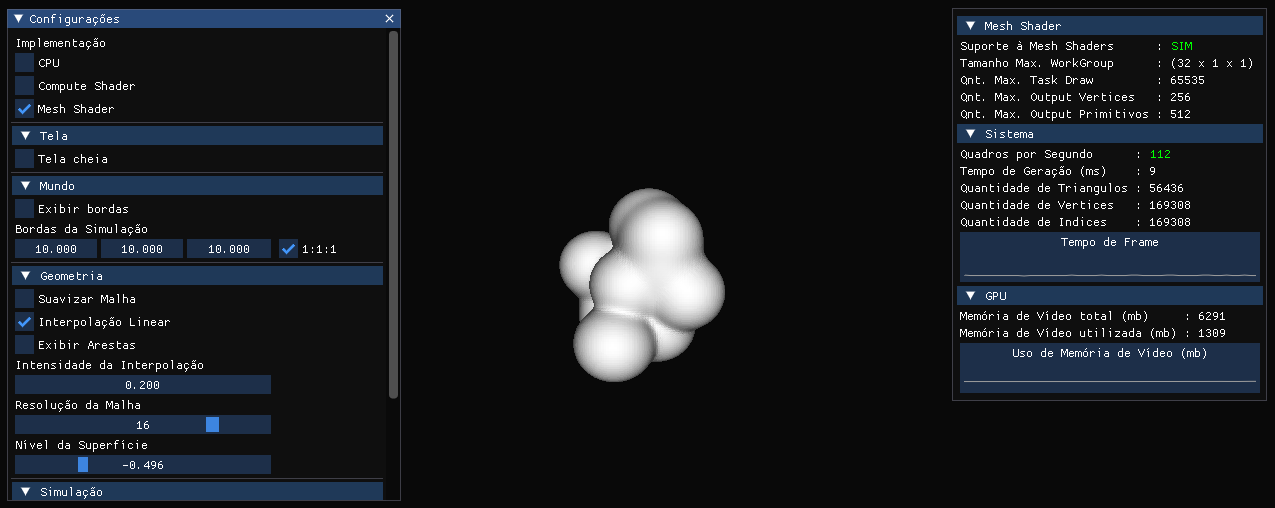
\includegraphics[width=1\textwidth]{imagens/InterfaceFerramenta.png}
\caption{Tela inicial da ferramenta desenvolvida para este estudo}
\label{fig:LABEL_FIG_MESH_SHADER_TOOL}
\end{figure}

\subsection{Funcionalidades}\label{sec:LABEL_FERRAMENTA_DESENVOLVIDA_FUNCIONALIDADES}
Nossa ferramenta é capaz observar se o computador que a executa possui suporte aos mesh shaders e de monitorar a utilização de recursos em tempo de execução. A figura \ref{fig:LABEL_FIG_FUNC_FERRAMENTA} ilustra a interface exibida durante a execução do programa. A tabela \ref{TBL:DESCRICAO_INFO_FERRAMENTA} descreve essas informações.

\begin{figure}
\centering
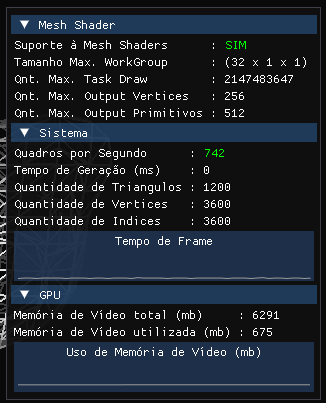
\includegraphics[width=0.5\textwidth]{imagens/FuncionalidadesFerramenta.png}
\caption{Tela inicial da ferramenta desenvolvida para este estudo}
\label{fig:LABEL_FIG_FUNC_FERRAMENTA}
\end{figure}

\begin{center}
\begin{table}
\begin{tabular}{|m{10em} | m{4em} | m{19em} |} 
 \hline
 Campo & Tipo & Descrição  \\
 \hline
Suporte à Mesh Shaders & Boolean & Verdadeiro se e somente se existe suporte ao OpenGL 4.6 e à extensão \textit{GL\_NV\_mesh\_shader} \\ \hline
Tamanho Max. WorkGroup & String & Quantidade máxima de Workgroups despachados por instância de Task/Mesh Shaders  \\ \hline
Qnt. Max. Task Draw & Integer & Quantidade máxima de instâncias de Mesh shaders instanciados por Task Shader   \\  \hline
Qnt. Max. Output Vértices & Integer & Quantidade máxima de vértices gerados por Workgroup \\  \hline
Qnt. Max. Output Primitives & Integer & Quantidade máxima de primitivos gerados por Workgroup \\  \hline
Quadros por Segundo & Integer & Quantidade de quadros (frames) renderizadas por segundo \\  \hline
Tempo de Geração (ms) & Integer & Tempo de geração da malha utilizando o algoritmo de Marching Cubes em milissegundos \\  \hline
Quantidade de Triângulos & Integer & Quantidade total de triângulos renderizados \\  \hline
Quantidade de Vértices & Integer & Quantidade total de vértices renderizados \\  \hline
Quantidade de Indices & Integer & Quantidade total de indices renderizados \\  \hline
Memória de video total (mb) & Integer & Capacidade total de memória de vídeo em mega bites \\  \hline
Memória de video utilizada (mb) & Integer & Quantidade de memória de vídeo utilizada em mega bites \\  \hline

\end{tabular}
\caption{Informações monitoradas durante a execução do programa}
\label{TBL:DESCRICAO_INFO_FERRAMENTA}
\end{table}
\end{center}

\section{Metodologia dos experimentos}\label{sec:LABEL_AMBIENTE_EXPERIMENTOS}

Visto que o objetivo do trabalho é estudar o comportamento do pipeline de renderização em contexto de aplicações em tempo real, os dados observados foram relacionados ao tempo de geração de frame para cada uma das seguintes implementações:

\begin{itemize}
    \item Em memória via CPU: a iteração sobre os pontos são feitas linearmente em memória principal diretamente pela CPU. O resultado do processo são os index e vertex buffers que são repassados para a esteira VGTs para renderização;
    \item Renderização indireta via compute shaders: os pontos são distribuídos entre as threads dos workgroups. Cada thread pode realizar seu processamento de forma completamente paralela das demais. O resultado do processo são os index e vertex buffers que são renderizados de forma indireta, conforme abordamos durante a Sessão \ref{sec:LABEL_FLUXO_DOS_DADOS}.;
    \item Renderização direta via mesh shaders: os pontos são distribuídos entre as threads dos workgroups. Cada thread pode realizar seu processamento de forma completamente paralela das demais. O resultado do processo são os index e vertex buffers repassados diretamente para a rasterização e renderização;
\end{itemize}

Todos os testes foram executados em um \textit{desktop} com processador Intel Core i5 10400f, 16 \textit{gibabytes} de RAM, placa de vídeo NVIDIA GeForce GTX 1660 Super e sistema operacional \textit{Windows 11}. 

\section{Resultados}\label{sec:LABEL_RESULTADOS}

\begin{figure}
\centering
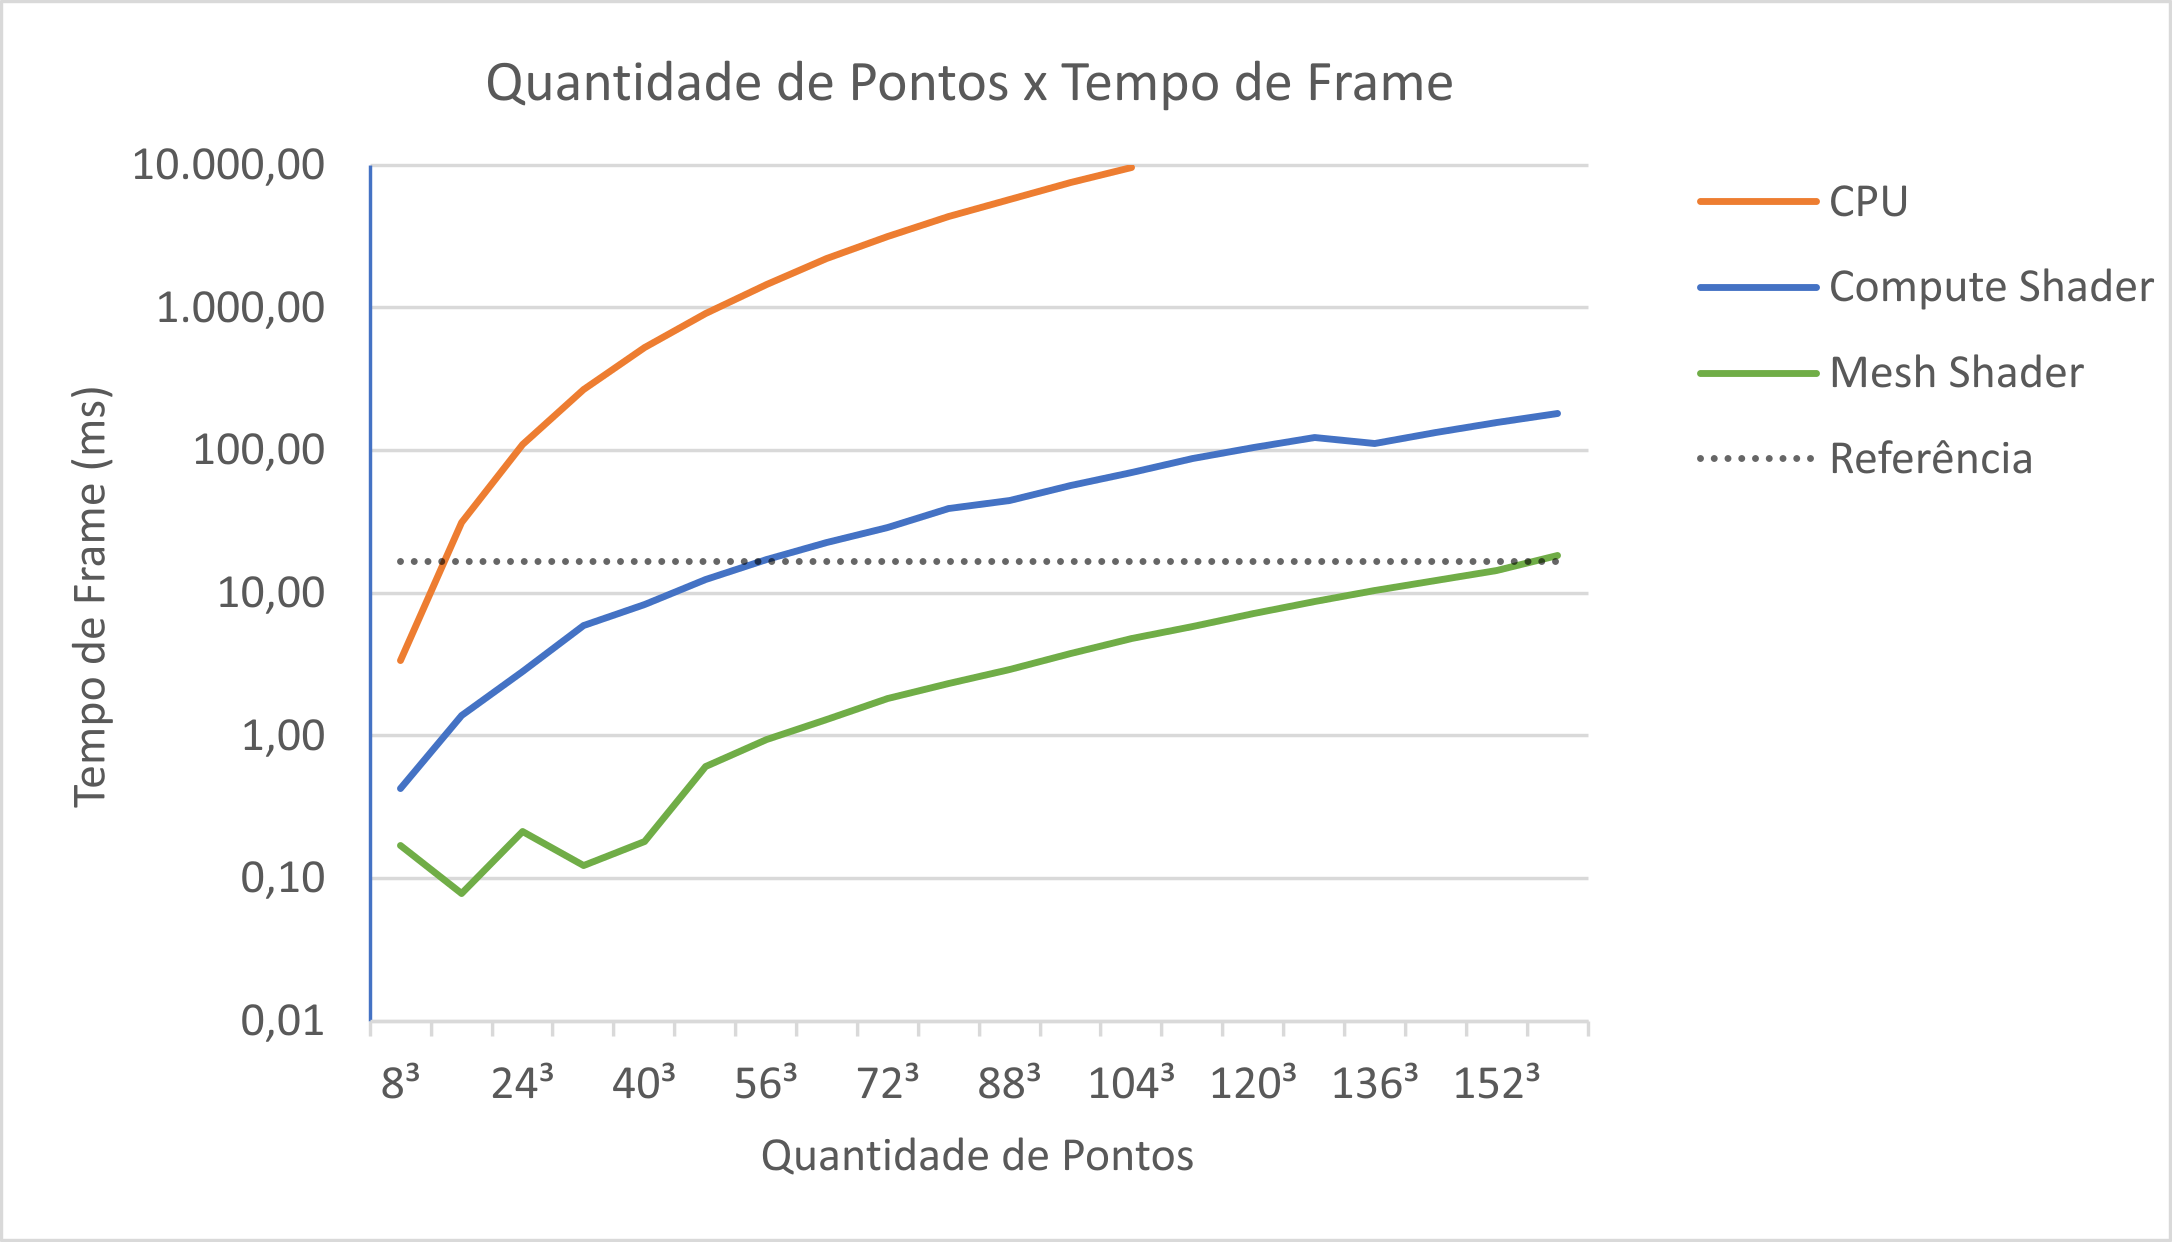
\includegraphics[width=1\textwidth]{imagens/PontosXTempoFrame.png}
\caption{Relação entre a quantidade de pontos e tempo de frame}
\label{fig:LABEL_FIG_PONTOS_X_TEMPO}
\end{figure}

Durante a execução do algoritmo utilizando em mesh shaders, conseguimos observar uma significativa redução no tempo de geração de frames em relação as demais implementações, se mantendo abaixo do limiar desejável de ~16,666 ms de tempo de frame até que a quantidade de pontos atingisse um total de $152^3$ pontos. A figura \ref{fig:LABEL_FIG_PONTOS_X_TEMPO} ilustra a diferença entre o tempo de geração de imagens entre as implementações. A visualização dos ganhos do uso de Mesh shaders em comparação aos compute shaders é detalhado pela Tabela \ref{TBL:TEMPO_FRAME_IMPL}. 

\begin{center}
\begin{table}
\begin{tabular}{|c | c | c | c |} 
 \hline
 Qnt. de Pontos & Compute Shaders (ms) & Mesh shaders (ms) & SpeedUp  \\
 \hline\hline
8³ & 0,424046 & 0,169582 & 2,5 \\ \hline
16³ & 1,377016 & 0,078685 & 17,5 \\ \hline
24³ & 2,808765 & 0,213918 & 13,1 \\ \hline
32³ & 5,886228 & 0,122899 & 47,9 \\ \hline
40³ & 8,252874 & 0,180791 & 45,6 \\ \hline
48³ & 12,484848 & 0,612670 & 20,4 \\ \hline
56³ & 17,285714 & 0,940276 & 18,4 \\ \hline
64³ & 22,793103 & 1,294455 & 17,6 \\ \hline
72³ & 28,800000 & 1,821869 & 15,8 \\ \hline
80³ & 39,000000 & 2,329283 & 16,7 \\ \hline
88³ & 44,647059 & 2,915858 & 15,3 \\ \hline
96³ & 56,357143 & 3,769663 & 15,0 \\ \hline
104³ & 70,250000 & 4,819277 & 14,6 \\ \hline
112³ & 87,375000 & 5,834586 & 15,0 \\ \hline
120³ & 105,222222 & 7,161017 & 14,7 \\ \hline
128³ & 122,857143 & 8,684211 & 14,1 \\ \hline
136³ & 111,125000 & 10,376238 & 10,7 \\ \hline
144³ & 133,000000 & 12,162162 & 10,9 \\ \hline
152³ & 156,250000 & 14,400000 & 10,9 \\ \hline
160³ & 181,073171 & 18,281250 & 9,9 \\ [1ex] \hline
\end{tabular}
\caption{Tempo de geração de frame durante a execução de marching cubes}
\label{TBL:TEMPO_FRAME_IMPL}
\end{table}
\end{center}

Em ambas as implementações não foi notado grandes variações quanto a quantidade de memória dedicada de vídeo foi alocada. Entretanto, a implementação em mesh shaders mostrou um uso mais estável do uso dos recursos. Conforme ilustrado na Figura \ref{fig:LABEL_USO3D_GPU}, onde o intervalo 1 representa a implementação em compute shaders e o intervalo 2 mesh shaders, a maior diferença observada foi em questão do uso dos mecanismo 3D da GPU, que chegou a $92\%$ em testes mais pesados em contraste da média de uso de aproximadamente $20\%$ vista em compute shaders.

Acreditamos que tais resultados sejam consequência da renderização indireta necessária em compute shaders. Parte do processamento é delegado da GPU para a CPU. Em cargas mais altas, a GPU se encontrava osciosa enquanto a CPU resgatava e repassava os SSBOs em forma de vertex e index buffers para alimentar a esteira VGTs.


\begin{figure}
\centering
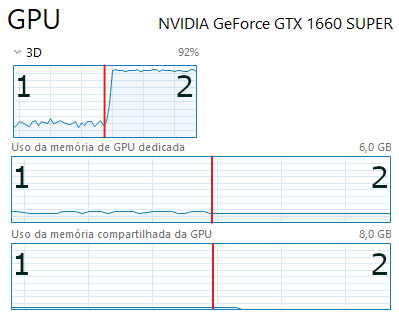
\includegraphics[width=0.75\textwidth]{imagens/Uso3DGPU.png}
\caption{Uso dos recursos da GPU durante a execução do algoritmo.}
\label{fig:LABEL_USO3D_GPU}
\end{figure}
